\documentclass[sn-nature]{sn-jnl}% Style for submissions to Nature Portfolio journals
%\documentclass[pdflatex,iicol]{sn-jnl}% Default with double column layout

\usepackage{graphicx}
\usepackage{multirow}
\usepackage{amsmath,amssymb,amsfonts}
\usepackage{amsthm}
\usepackage{mathrsfs}
\usepackage[title]{appendix}
\usepackage{xcolor}
\usepackage{textcomp}
\usepackage{manyfoot}
\usepackage{booktabs}
\usepackage{algorithm}
\usepackage{algorithmicx}
\usepackage{listings}
\usepackage{caption}
\usepackage{subcaption}


\begin{document}

\title[Article Title]{A coherent stimulated phonon spectrometer}

\author*[1,2]{\fnm{Joel} \sur{N. Johnson}}\email{joel.johnson@nau.edu}

\author[3]{\fnm{Peter} \sur{T. Rakich}}

\author[4]{\fnm{Co} \sur{Authors}}

\author*[1,2]{\fnm{Ryan} \sur{O. Behunin}}\email{ryan.behunin@nau.edu}

\affil*[1]{\orgdiv{Department of Applied Physics and Materials Science}, \orgname{Northern Arizona University}, \orgaddress{\city{Flagstaff}, \postcode{86011}, \state{AZ}, \country{USA}}}

\affil[2]{\orgname{Center for Materials Interfaces in Research and Applications}, \orgaddress{\city{Flagstaff}, \postcode{86011}, \state{AZ}, \country{USA}}}

\affil[3]{\orgdiv{Department of Applied Physics}, \orgname{Yale University}, \orgaddress{\city{New Haven}, \postcode{06520}}, \state{CT}, \country{USA}}

\affil[4]{\orgdiv{Department}, \orgname{Organization}, \orgaddress{\street{Street}, \city{City}, \postcode{610101}, \state{State}, \country{Country}}}

\abstract{Brillouin scattering is the inelastic scattering of light with sound, or, equivalently, from acoustic phonons. A spontaneous Brillouin scattering process is the scattering of light with specifically the thermodynamic fluctuations in a material, providing information about the material's thermal properties within its various mechanical modes. Sufficient optical power can elevate this spontaneous process into a stimulated one, known as stimulated Brillouin scattering: a regime in which the optical fields themselves are augmenting the optical properties of the material, often greatly enhancing the optomechanical response of the material in a self-reinforcing Stokes process. [] We present a coherent stimulated phonon spectrometer that utilizes a pump-probe design to measure Brillouin scattering with sub-10femptowatt sensitivity. By employing three mechanisms to segregate the pump and probe light, we achieve sub-10 femptowatt sensitivity, enabling phonon spectroscopy on scales not previously possible. We demonstrate the capabilities of the instrument by observing Brillouin scattering in 1 centimeter and 1 millimeter of UHNA3 fiber, and 4 millimeters of bulk carbon disulfide, each at room temperature with sub-Watt optical power. This instrument paves new avenues for materials characterization and the development of novel nano-acousto-optic devices.}

\keywords{Brillouin, femptowatt, nano-acousto-optic, phonon spectrometer}

\maketitle

\section{Introduction}
\label{Intro}

[better first sentence] Brillouin scattering is a [less definition-y] fundamental process in which light interacts with acoustic phonons in a material, leading to a shift in the scattered light's frequency. [annihilation of ...] This process has been extensively studied for its potential applications in fields such as sensing, communications, and the development of optomechanical devices. However, [spontaneous, stimulated, would be nice if dedicated Stokes pump, but such an instrument would need to overcome the conflation of Stokes pump and retro-reflected Stokes-shifted probe signal..] conventional methods for measuring Brillouin scattering have been limited by their sensitivity, hindering the exploration of new phenomena and applications at the nanoscale. In this paper, we introduce a coherent stimulated phonon spectrometer that overcomes these limitations, enabling measurements with sub-10 femptowatt sensitivity.


\section{Results}\label{Results}

\begin{figure}[t]
\centering
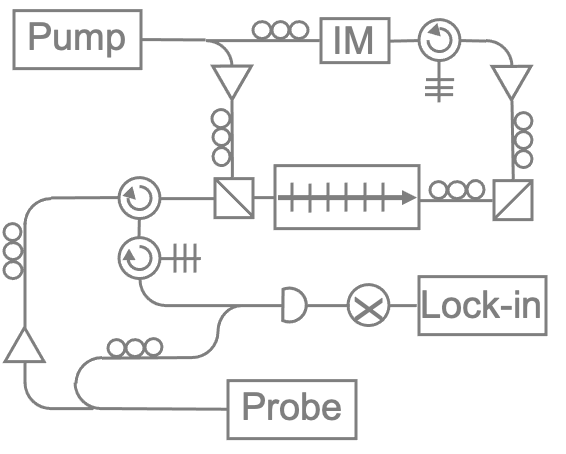
\includegraphics[width=.45\textwidth]{CABS.png}
\caption{CABS design diagram}\label{fig:CABS}
\end{figure}

In Fig. \ref{fig:CABS}, a pump and Stokes signal is synthesized from a single tunable laser source for coherent stimulation of the sample. The pump signal ($\omega_{Pump}$) is amplified by an erbium-doped fiber amplifier (EDFA) and passed through a variable optical attenuator (VOA). The output is then polarization-controlled to reflect at a polarizing beam splitter (PBS) for injection into the sample. For Stokes synthesis, an AC signal ($\Omega$) is supplied to an intensity modulator with carrier frequency nulled and a tunable filter is used to select one side band output ($\omega_{Pump} - \Omega$). This Stokes signal is then amplified by an EDFA, passed through a VOA, and polarization-controlled to reflect at a second PBS for couter-propagating injection into the sample.

A separate tunable laser ($\omega_{Probe} = \omega_{Pump} + $) is used to synthesize the probe and local oscillator (LO). Probe light is amplified by an EDFA and fed through a VOA. A polarization controller aligns the polarization axis of the probe light for transmission through the first PBS and copropagation with the pump into the sample. Backscattered probe light retraces through the first PBS while the orthogonally polarized Stokes light is diverted along a different path. The backscattered signal ($\omega_{Signal} = \omega_{Probe} + \Omega$) then routes through two subsequent circulators for spectral filtering by a 5 GHz bandpass tunable filter which passes the frequency-shifted probe light while rejecting any reflected probe light as well as any reflected, transmitted, or backscattered light from the pump and Stokes that was not diverted by the PBS. The filtered signal combines via a 99-1 splitter with the frequency upshifted LO ($\omega_{Probe} + 40 MHz$) which has been polarization-controlled to be in parallel with the signal polarization. This heterodyned signal ($\Omega + 40 MHz$) is then captured by a photodiode detector, heterodyned again with an AC signal ($\Omega - 5 MHz$) by a radio frequency (RF) mixer, and read into a lock-in amplifier for data collection. Both AC signals, for the RF mixer and Stokes synthesis, are swept together when taking a measurement so as to maintain a constant 45 MHz lock-in frequency.

We consider two example targets to demonstrate the capabilities of the instrument, one fiber-coupled and one bulk material. Fig. \ref{fig:1cmUHNA3} shows the spectra captured for 1 cm of UHNA3 fiber. The spectral shape is that of the expected lorentzian function, with the peak ([9.18 GHz]) indicating the Brillouin resonance frequency and the FWHM ([~80 MHz]) indicating the dissipation rate of the fiber. [comparison to regular SBS for some measurable length of UHNA3?]\\

\begin{figure}[t]
  \centering
  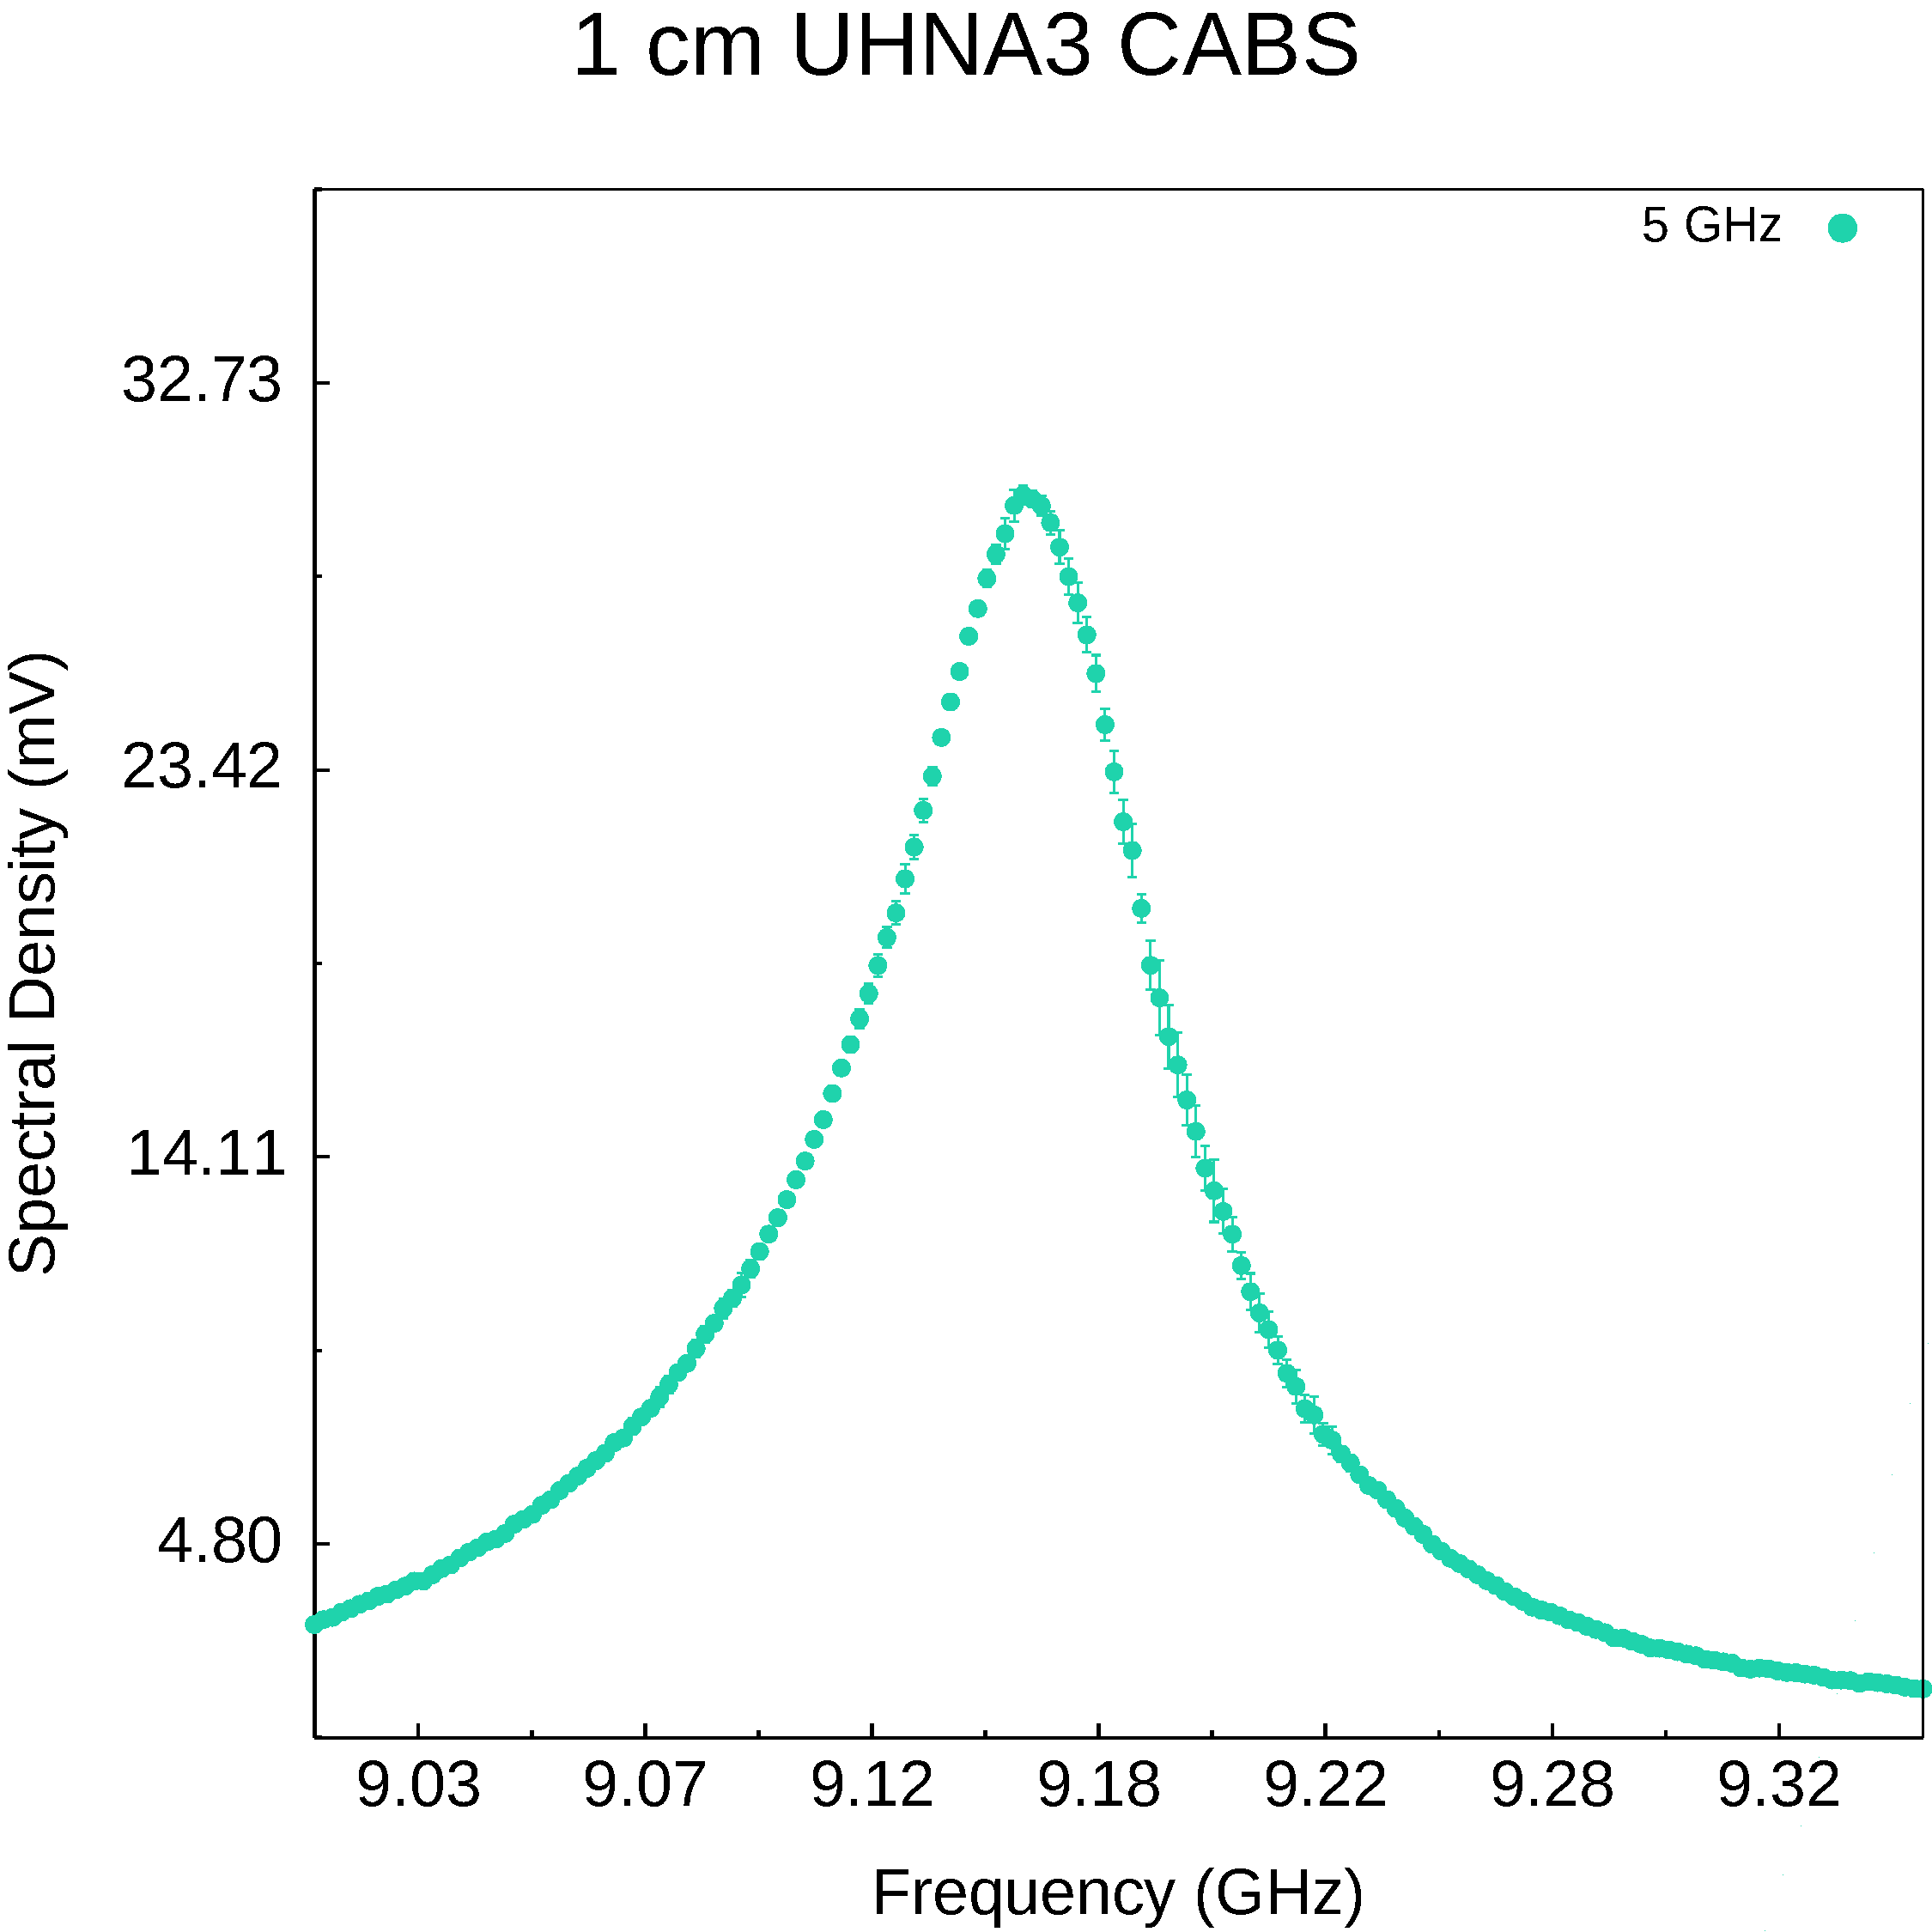
\includegraphics[width=.45\textwidth]{1cmUHNA3.pdf}
  \caption{1cm UHNA3 [needs fit]}\label{fig:1cmUHNA3}
\end{figure}

\begin{figure}[t]
  \centering
  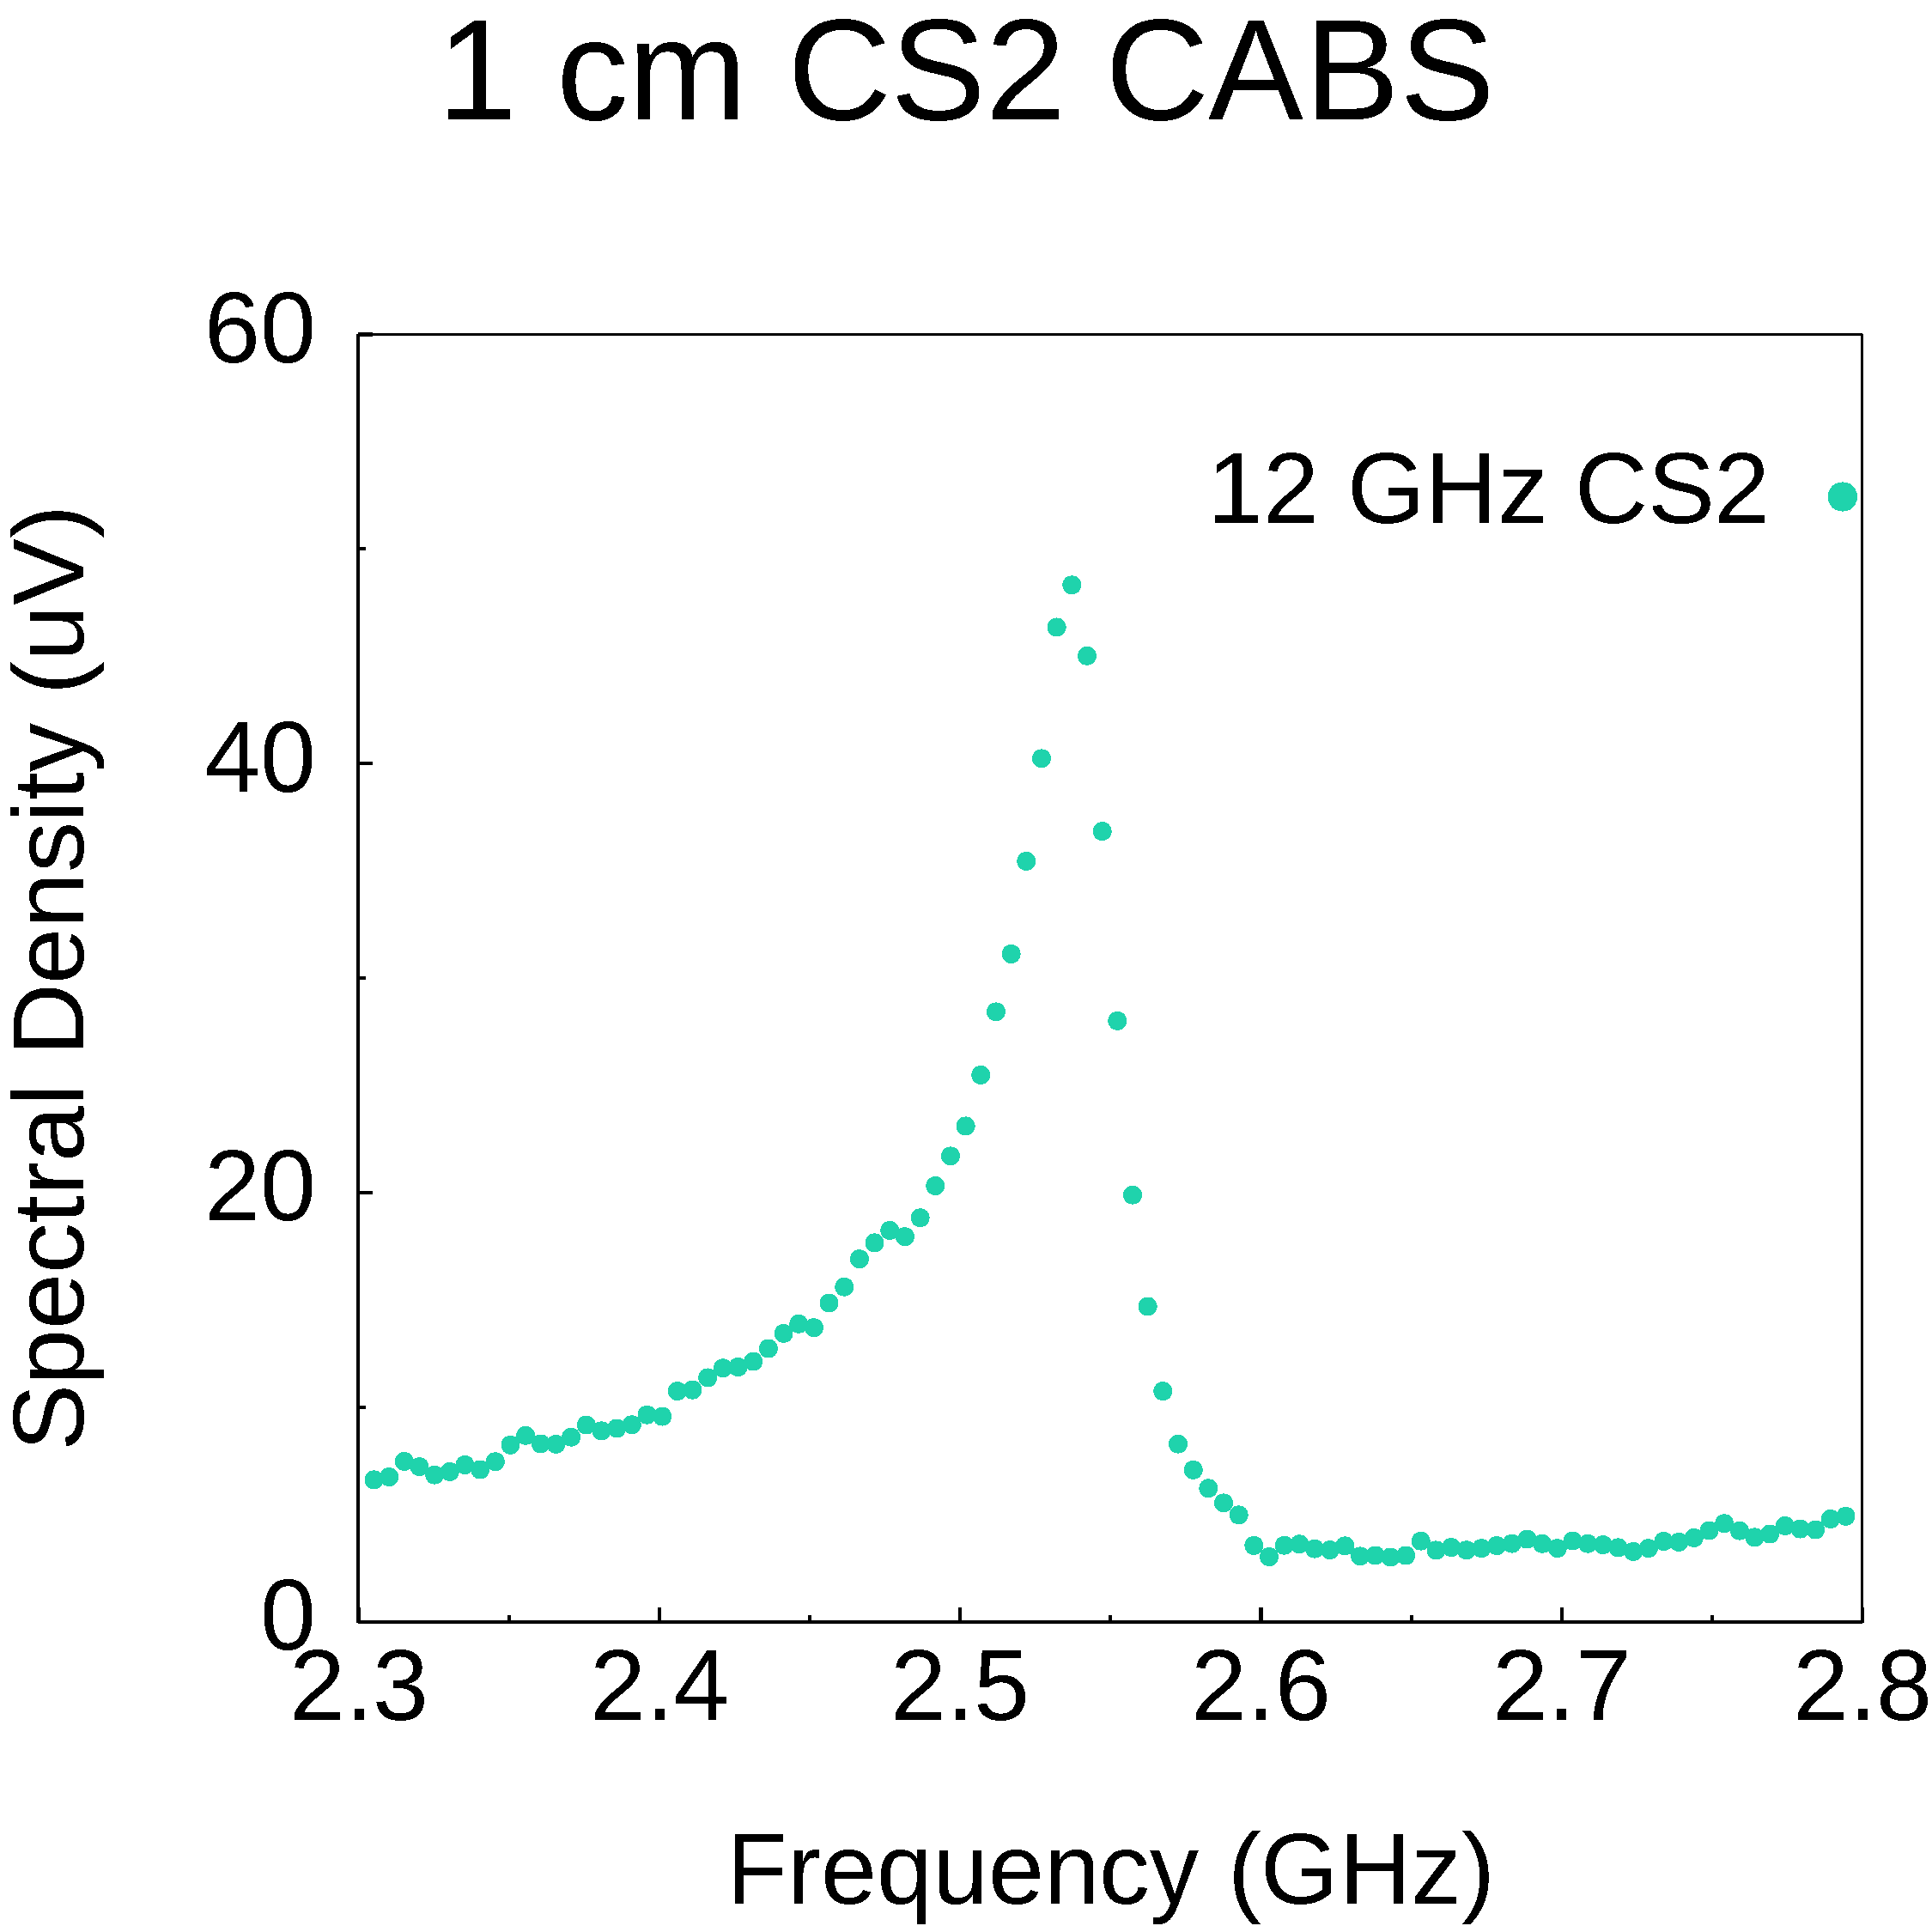
\includegraphics[width=.45\textwidth]{4mmCS2.pdf}
  \caption{4mm CS2}\label{fig:4mmCS2}
\end{figure}

Fig. \ref{fig:} shows the spectral measurements achieved by the instrument, overlaid with finite-difference simulation data. In Fig. \ref{fig:} we see the expected lorentzian spectral shape in good alignment with simulation data for guided longitudinal modes in the core of the UHNA3 fiber. In Fig. \ref{fig:}, however, we see a distortion of this lorentzian shape. This is expected for partially unguided longitudinal modes, such as is the case for a bulk liquid filling the volume of a ...

Fig. \ref{fig:1cmUHNA3} shows a measurement of 1cm of UHNA3 fiber.

First, we measured Brillouin scattering in a 1-centimeter-long UHNA3 fiber at room temperature and with sub-Watt optical power (Fig. \ref{fig:}). Figure \ref{fig:}, clearly displays the Brillouin scattering features with remarkable signal-to-noise ratio, highlighting the effectiveness of our apparatus in isolating the backscattered probe light. This observation serves as one of the main showcases of the instrument's capability.

Next, we performed Brillouin scattering measurements on a 4-millimeter-thick bulk carbon disulfide sample in a free-space optics arrangement. The observed spectrum, presented in Figure 2, exhibits well-resolved Brillouin scattering peaks. This successful measurement in a bulk sample demonstrates the versatility and adaptability of our instrument to various experimental configurations, further emphasizing the instrument's capability.

Lastly, we conducted a measurement in a 1-millimeter-long UHNA3 fiber under low-power conditions, with only 10 microwatts of power at the sample. Despite the reduced sample length and low power, the instrument's sensitivity allowed us to observe distinct Brillouin scattering features in the spectrum, as illustrated in Figure 3. This result underscores the potential of our spectrometer for nanoscale measurements and serves as a demonstration of the instrument's sensitivity, defining the sensitivity floor of the apparatus.

These three observations collectively showcase the high sensitivity, broad applicability, and impressive capabilities of our coherent stimulated phonon spectrometer in measuring Brillouin scattering across different sample types, scales, and power levels.

\begin{figure}[t]
\centering
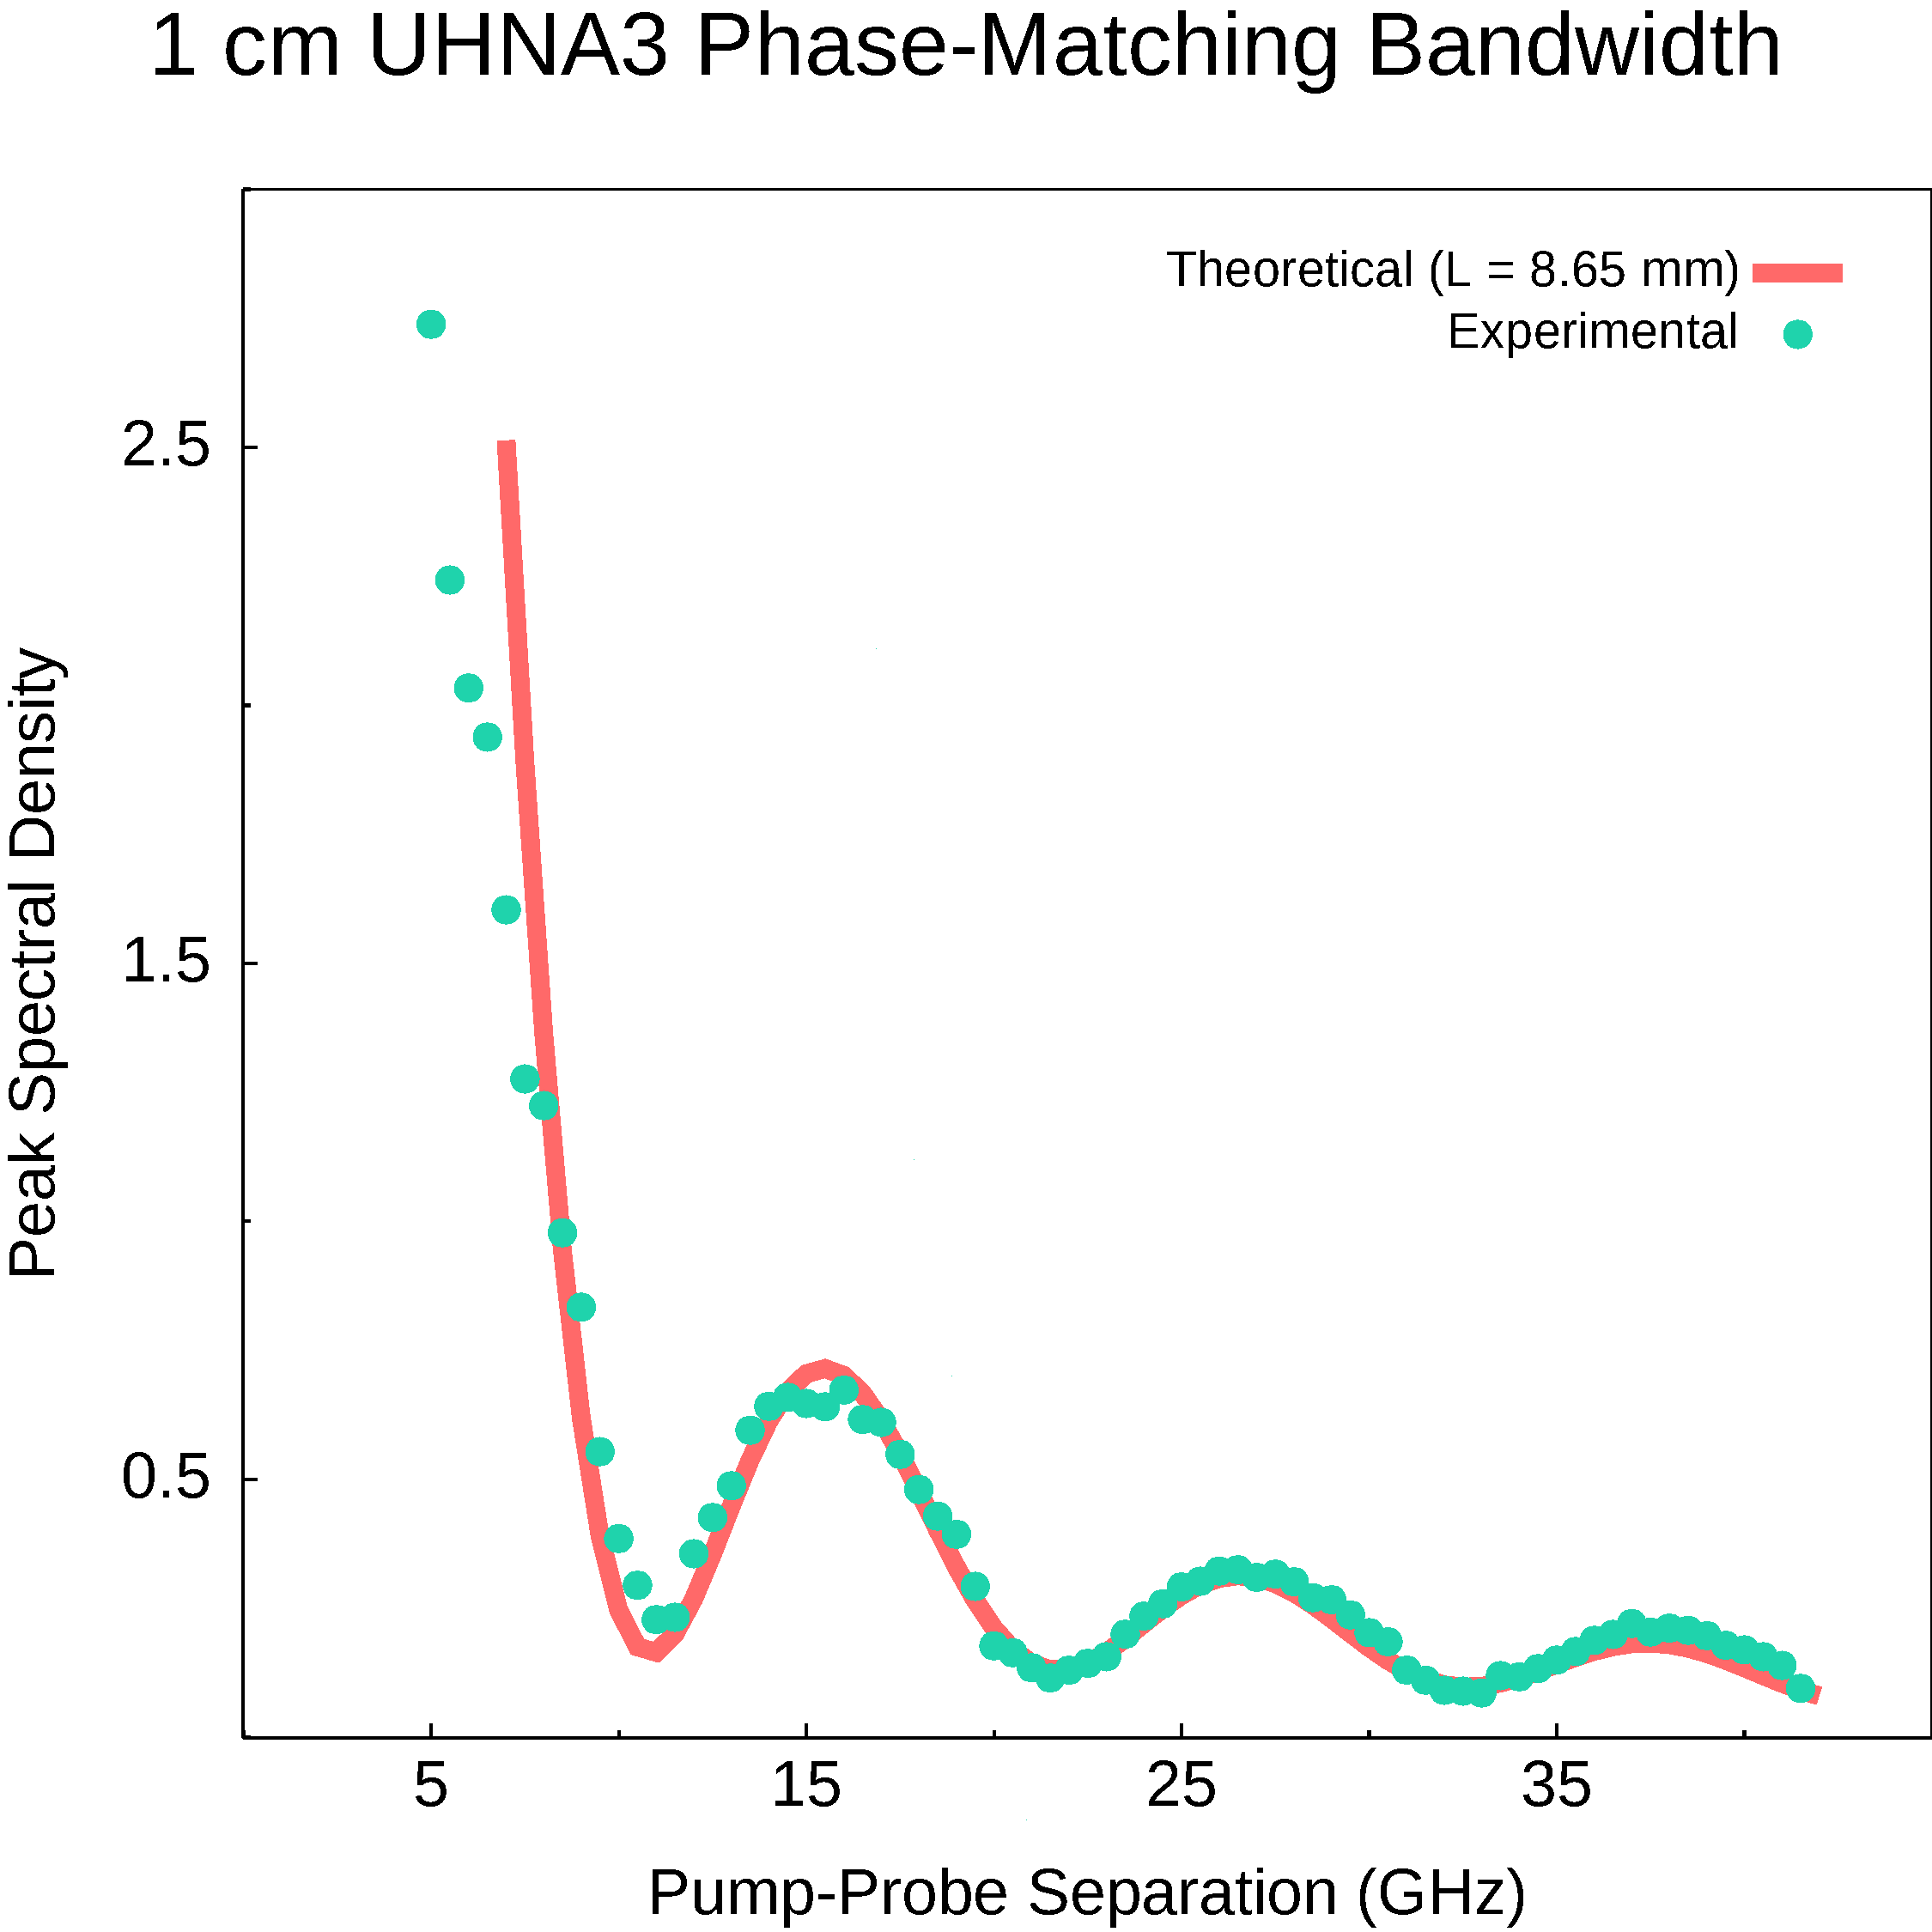
\includegraphics[width=.45\textwidth]{Phase-Match.pdf}
\caption{Phase-matching sinc func}\label{fig:Phase-Match}
\end{figure}

\section{Theory}\label{Theory}

Here we derive the coupled wave equations that describe coherent stimulated Brillouin scattering involving a pump, Stokes, probe, and backscattered optical field given respectively by

\begin{equation}
    \tilde{E}_{P}(z,t) = A_{P}e^{i(k_{P}z - \omega_{P}t)} + c.c.
    \label{eq:Pump optical field}
\end{equation}
\begin{equation}
    \tilde{E}_{S}(z,t) = A_{S}e^{i(k_{S}z - \omega_{S}t)} + c.c.
    \label{eq:Stokes optical field}
\end{equation}
\begin{equation}
    \tilde{E}_{Pr}(z,t) = A_{Pr}e^{i(k_{Pr}z - \omega_{Pr}t)} + c.c.
    \label{eq:Probe optical field}
\end{equation}
\begin{equation}
    \tilde{E}_{Sig}(z,t) = A_{Sig}e^{i(k_{Sig}z - \omega_{Sig}t)} + c.c.
    \label{eq:Signal optical field}
\end{equation}
\\
\noindent and a common acoustic field given by
\begin{equation}
    \tilde{\rho}(z,t) = \rho_{0} + \rho(z,t)e^{i(qz - \Omega t)} + c.c.,
    \label{eq:acoustic field}
\end{equation}
\noindent where $\Omega = \omega_{P} - \omega_{S}$ and $q = k_{P} - k_{S} = 2k_{P}$.
\subsection{Acoustic Field}
We start by assuming that the material obeys the acoustic wave equation,
\begin{equation}
    \frac{\partial^{2}\tilde{\rho}}{\partial t^{2}} - \Gamma^{\prime}\nabla^{2}\frac{\partial\tilde{\rho}}{\partial t} - v^{2}\nabla^{2}\tilde{\rho} = \nabla\cdot\vec{f},
    \label{eq:acoustic wave equation}
\end{equation}
\noindent where $v$ is the sound speed in the material and $\Gamma^{\prime}$ is a damping parameter given by
\begin{equation}
    \Gamma^{\prime} = \frac{1}{\rho}\left[\frac{4}{3}\eta_{s} + \eta_{b} + \frac{\kappa}{C_{p}}(\gamma - 1)\right],
\end{equation}
\noindent where $\eta_{s}$ and $\eta_{b}$ are the shear and bulk viscosity coefficients of the material, respectively. The source term on the right side of Eq. (\ref{eq:acoustic wave equation}) is the divergence of the electrostrictive force:
\begin{equation}
    \vec{f} = \nabla p_{st} = \nabla \cdot \left[-\frac{1}{2}\epsilon_{0}\gamma_{e}\left(\langle\tilde{E}_{P} \cdot \tilde{E}_{S}\rangle + \langle\tilde{E}_{Pr} \cdot \tilde{E}_{Sig}\rangle\right)\right],
\end{equation}
which yields, after applying the slowly varying amplitude approximation,
\begin{equation}
    \nabla\cdot\vec{f} = \epsilon_{0}\gamma_{e}q^{2}(A_{P}A_{S}^{*} + A_{Pr}A_{Sig}^{*}e^{i\Delta kz}),
\end{equation}
\\
Where $\Delta k = (k_{Pr} - k_{Sig}) - (k_{P} - k_{S})$ is the phase mismatch between the four optical fields. Only two electrostrictive terms survive terms after accounting for the orthogonal polarization of the pump and Stokes fields with respect to that of the probe and backscattered signal. Inserting this electrostrictive force term and the acoustic field (Eq. (\ref{eq:acoustic field})) into Eq. (\ref{eq:acoustic wave equation}) and assuming a slowly varying acoustic amplitude we find
\begin{equation}
    -2i\Omega\frac{\partial\rho}{\partial t} - \Gamma^{\prime}2iq^{2}\Omega\rho - 2iqv^{2}\frac{\partial\rho}{\partial z} = \epsilon_{0}\gamma_{e}q^{2}(A_{P}A_{S}^{*} + A_{Pr}A_{Sig}^{*}e^{i\Delta kz}),
\end{equation}
which can be restated in terms of the Brillouin linewidth, $\Gamma_{B} = q^{2}\Gamma^{\prime}$, as
\begin{equation}
    -2i\Omega\frac{\partial\rho}{\partial t} - 2i\Omega\Gamma_{B}\rho - 2iqv^{2}\frac{\partial\rho}{\partial z} = \epsilon_{0}\gamma_{e}q^{2}(A_{P}A_{S}^{*} + A_{Pr}A_{Sig}^{*}e^{i\Delta kz}).
    \label{eq:in terms of Brillouin linewidth}
\end{equation}
Given the phonon dispersion relations $\Omega_{B} = |q_{B}|v$ and $\Omega^{2} = q^{2}\left(v^{2} - i\Omega\Gamma^{\prime}\right)$, Eq. (\ref{eq:in terms of Brillouin linewidth}) can be rewritten as
\begin{equation}
    -2i\Omega\frac{\partial\rho}{\partial t} + \left(\Omega^{2} - \Omega^{2} - i\Omega\Gamma_{B}\right)\rho - 2iqv^{2}\frac{\partial\rho}{\partial z} = \epsilon_{0}\gamma_{e}q^{2}(A_{P}A_{S}^{*} + A_{Pr}A_{Sig}^{*}e^{i\Delta kz}).
    \label{eq:in terms of Omega_B}
\end{equation}
We take the common assumption that the phonon propagation distance is small compared to the distance over which the source term varies significantly, which allows the spatial derivative term in Eq. (\ref{eq:in terms of Omega_B}). We further assume steady-state conditions such that the time derivative term also vanishes, leaving
\begin{equation}
    (\Omega^{2}_{B} - \Omega^{2} - i\Omega\Gamma_{B})_{\rho} = \epsilon_{0}\gamma_{e}q^{2}(A_{P}A_{S}^{*} + A_{Pr}A_{Sig}^{*}e^{i\Delta kz}).
\end{equation}
We thus find the acoustic field amplitude to be
\begin{equation}
    \rho(z,t) = \epsilon_{0}\gamma_{e}q^{2}\frac{A_{P}A_{S}^{*} + A_{Pr}A_{Sig}^{*}e^{i\Delta kz}}{\Omega_{B}^{2} - \Omega^{2} - i\Omega\Gamma_{B}}.
    \label{eq:Acoustic field amplitude}
\end{equation}
\subsection{Optical Fields}
We now turn to the spatial evolution of the optical fields, described by the wave equation,

\begin{equation}
    \frac{\partial^{2}\tilde{E}_{i}}{\partial z^{2}} - \frac{n^{2}}{c^{2}}\frac{\partial^{2}\tilde{E}_{i}}{\partial t^{2}} = \frac{1}{\epsilon_{0}c^{2}}\frac{\partial^{2}\tilde{P}_{i}}{\partial t^{2}},
    \label{eq:Wave equation}
\end{equation}
\\
where i denotes the four optical fields, namely: pump, Stokes, probe, and backscattered signal. The total nonlinear polarization that gives rise to the source term in the wave equation is given by
\begin{equation}
    \tilde{P} = \epsilon_{0}\Delta\chi\tilde{E} = \epsilon_{0}\Delta\epsilon\tilde{E} = \epsilon_{0}\rho^{-1}\gamma_{e}\tilde{\rho}\tilde{E}.
\end{equation}
The parts of $\tilde{P}$ that can act as phase-matched source terms for the optical fields are
\begin{equation}
    \tilde{P}_{P} = p_{P}e^{i(k_{P}z - \omega_{P} t)} + c.c. = \frac{1}{2}\epsilon_{0}\rho_{0}^{-1}\gamma_{e}\rho A_{S}e^{i(k_{P}z - \omega_{P} t)}
    \label{eq:Pump phase-matched source term}
\end{equation}
\begin{equation}
    \tilde{P}_{S} = p_{S}e^{i(-k_{S}z - \omega_{S} t)} + c.c. = \frac{1}{2}\epsilon_{0}\rho_{0}^{-1}\gamma_{e}\rho^{*} A_{P}e^{i(-k_{S}z - \omega_{S} t)}
    \label{eq:Stokes phase-matched source term}
\end{equation}
\begin{equation}
    \tilde{P}_{Pr} = p_{Pr}e^{i(k_{Pr}z - \omega_{Pr} t)} + c.c. = \frac{1}{2}\epsilon_{0}\rho_{0}^{-1}\gamma_{e}\rho A_{Sig}e^{i(k_{Pr}z - \omega_{Pr} t)}e^{i\Delta kz}
    \label{eq:Probe phase-matched source term}
\end{equation}
\begin{equation}
    \tilde{P}_{Sig} = p_{Sig}e^{i(-k_{Sig}z - \omega_{Sig} t)} + c.c. = \frac{1}{2}\epsilon_{0}\rho_{0}^{-1}\gamma_{e}\rho^{*} A_{Pr}e^{i(-k_{Sig}z - \omega_{Sig} t)}e^{-i\Delta kz}.
    \label{eq:Signal phase-matched source term}
\end{equation}
\\
Inserting the optical fields (Eqs. \ref{eq:Pump optical field}-\ref{eq:Signal optical field}) and phase-matched source terms (Eqs. \ref{eq:Pump phase-matched source term}-\ref{eq:Signal phase-matched source term}) into Eq. (\ref{eq:Wave equation}), we obtain
\begin{equation}
    \frac{\partial A_{P}}{\partial z} + \frac{n}{c}\frac{\partial A_{P}}{\partial t} = \frac{i\omega_{P}\gamma_{e}}{2nc\rho_{0}}\rho A_{2}
\end{equation}
\begin{equation}
    -\frac{\partial A_{S}}{\partial z} + \frac{n}{c}\frac{\partial A_{S}}{\partial t} = \frac{i\omega_{S}\gamma_{e}}{2nc\rho_{0}}\rho^{*}A_{P}
\end{equation}
\\
\begin{equation}
    \frac{\partial A_{Pr}}{\partial z} + \frac{n}{c}\frac{\partial A_{Pr}}{\partial t} = \frac{i\omega_{Pr}\gamma_{e}}{2nc\rho_{0}}\rho A_{Sig}
\end{equation}
\\
\begin{equation}
    -\frac{\partial A_{Sig}}{\partial z} + \frac{n}{c}\frac{\partial A_{Sig}}{\partial t} = \frac{i\omega_{Sig}\gamma_{e}}{2nc\rho_{0}}\rho^{*}A_{Pr}
\end{equation}
\\
We again assume steady-state conditions, allowing the time derivative term to be dropped. Plugging in the acoustic field amplitude (Eq. \ref{eq:Acoustic field amplitude}), we arrive at the coupled-amplitude wave equations for the optical fields,
\begin{equation}
    \frac{\partial A_{P}}{\partial z} = \frac{i\epsilon_{0}\omega_{P} q^{2}\gamma_{e}^{2}}{2nc\rho_{0}}\frac{A_{P}|A_{S}|^{2} + A_{Pr}A_{Sig}^{*}A_{S}e^{i\Delta kz}}{\Omega_{B}^{2} - \Omega^{2} - i\Omega\Gamma_{B}}
\end{equation}
\begin{equation}
    \frac{\partial A_{S}}{\partial z} = -\frac{i\epsilon_{0}\omega_{S} q^{2}\gamma_{e}^{2}}{2nc\rho_{0}}\frac{|A_{P}|^{2}A_{S}^{*} + A_{Pr}A_{Sig}^{*}A_{P}e^{i\Delta kz}}{\Omega_{B}^{2} - \Omega^{2} - i\Omega\Gamma_{B}}
\end{equation}
\\
\begin{equation}
    \frac{\partial A_{Pr}}{\partial z} = \frac{i\epsilon_{0}\omega_{Pr} q^{2}\gamma_{e}^{2}}{2nc\rho_{0}}\frac{A_{P}A_{S}^{*}A_{Sig} + A_{Pr}|A_{Sig}|^{2}e^{i\Delta kz}}{\Omega_{B}^{2} - \Omega^{2} - i\Omega\Gamma_{B}}
\end{equation}
\\
\begin{equation}
    \frac{\partial A_{Sig}}{\partial z} = -\frac{i\epsilon_{0}\omega_{S} q^{2}\gamma_{e}^{2}}{2nc\rho_{0}}\frac{A_{P}A_{S}^{*}A_{Pr} + |A_{Pr}|^{2}A_{Sig}^{*}e^{i\Delta kz}}{\Omega_{B}^{2} - \Omega^{2} - i\Omega\Gamma_{B}}
    \label{eq:Signal coupled-amplitude wave equation}
\end{equation}
\\
Integrating Eq. \ref{eq:Signal coupled-amplitude wave equation} along the effective length gives the amplitudes of each optical field,
\\
\begin{equation}
  A_{P} = \frac{i\epsilon_{0}\omega q^{2}\gamma_{e}^{2}}{2nc\rho_{0}}\frac{A_{P}|A_{S}|^{2} + A_{Pr}A_{Sig}^{*}A_{S}}{\Omega_{B}^{2}-\Omega^{2}-i\Omega\Gamma_{B}} \frac{e^{-i\Delta kL}-1}{\Delta k},
\end{equation}
\\
\begin{equation}
  A_{S} = -\frac{i\epsilon_{0}\omega q^{2}\gamma_{e}^{2}}{2nc\rho_{0}}\frac{|A_{P}|^{2}A_{S}^{*} + A_{Pr}A_{Sig}^{*}A_{P}}{\Omega_{B}^{2}-\Omega^{2}-i\Omega\Gamma_{B}} \frac{e^{-i\Delta kL}-1}{\Delta k},
\end{equation}
\\
\begin{equation}
  A_{Pr} = -\frac{i\epsilon_{0}\omega q^{2}\gamma_{e}^{2}}{2nc\rho_{0}}\frac{A_{P}A_{S}^{*}A_{Sig} + A_{Pr}|A_{Sig}|^{2}}{\Omega_{B}^{2}-\Omega^{2}-i\Omega\Gamma_{B}} \frac{e^{-i\Delta kL}-1}{\Delta k},
\end{equation}
\\
\begin{equation}
  A_{Sig} = -\frac{i\epsilon_{0}\omega q^{2}\gamma_{e}^{2}}{2nc\rho_{0}}\frac{A_{P}A_{S}^{*}A_{Pr} + |A_{Pr}|^{2}A_{Sig}^{*}}{\Omega_{B}^{2}-\Omega^{2}-i\Omega\Gamma_{B}} \frac{e^{-i\Delta kL}-1}{\Delta k}.
\end{equation}
\\
The intensity of the backscattered signal is then given by the square of the magnitude of its amplitude,
\\
\begin{equation}
  I_{Sig} = \frac{\epsilon_{0}^{2}\omega^{2}q^{4}\gamma_{e}^{4}}{4n^{2}c^{2}\rho_{0}^{2}}\frac{I_{P}I_{S}I_{Pr}}{(\Omega_{B} - \Omega)^{4} - \Omega^{2}\Gamma_{B}^{2}}L^{2}sinc^{2}\left(\frac{\Delta kL}{2}\right)
\end{equation}
\\
Here we have taken the real part and dropped the very small terms containing the signal amplitude. Defining the intensities as $I_{i} = 2n\epsilon_{0}cA_{i}A_{i}^{*}$, the backscattered signal intensity is reduced to [see green writing to far right in onenote coupled wave equations of CABS]

To find the power of the backscattered signal, we would integrate this intensity over the effective area. Approximated for fiber as $\pi r^{2}$ where r is the effective mode field diameter, this becomes
\\
\begin{equation}
  P_{Sig} = \pi r^{2}\frac{\epsilon_{0}^{2}\omega^{2}q^{4}\gamma_{e}^{4}}{4n^{2}c^{2}\rho_{0}^{2}}\frac{P_{P}P_{S}P_{Pr}}{(\Omega_{B} - \Omega)^{4} - \Omega^{2}\Gamma_{B}^{2}}L^{2}sinc^{2}\left(\frac{\Delta kL}{2}\right).
\end{equation}




\bibliography{sn-bibliography}
%\bibliographystyle{plain}

\end{document}
